% Load LaTeX and package
\documentclass[11pt, xcolor=x11names,compress]{beamer}
\usepackage[utf8]{inputenc}
\usepackage{mathtools}  % for paired delimiters 
\usepackage{mathrsfs}   % for script capitals
\usepackage{amsmath}
\usepackage{amssymb}
\usepackage{amsfonts}

\usepackage[dvipsnames]{xcolor} % for color
\usepackage{ragged2e} % for text alignment
\usepackage{dsfont} % for sepecial font (mathds)

\usepackage[labelformat=empty]{caption}

\usepackage{natbib}
\bibliographystyle{abbrvnat}
% Customize theme attributes
\setbeamertemplate{headline}[default]
%% Hide navigation symbols
\setbeamertemplate{navigation symbols}{}
%%\mode<beamer>{\setbeamertemplate{blocks}[rounded][shadow=true]} %for block
%% Outer theme
\useoutertheme{infolines}
\useoutertheme[subsection=false]{miniframes}

%% Inner theme
\useinnertheme{}

% Define template colors
\usecolortheme{rose}
%\usecolortheme{default}

\definecolor{UniColor}{RGB}{0,0, 255}
\setbeamercolor{structure}{bg=white, fg=UniColor}
\setbeamercolor{title}{bg = white, fg = UniColor}
\setbeamercolor{author}{bg = white, fg = UniColor}

\DeclareMathOperator{\Var}{\text{Var}}
\DeclareMathOperator{\E}{\text{E}}
\DeclareMathOperator{\Cov}{\text{Cov}}
\DeclareMathOperator{\Corr}{\text{Corr}}

%------------------------------------------------------------
%This block of code defines the information to appear in the
%Title page



\title [ECON 4003: Empirical Exercise 3.2]{ECON 4003 Econometrics I}

\vspace{10mm}

\author[]{Empirical Exercise 3.2}
\date{b\textit{y Duong Trinh}}

%End of title page configuration block
%---------------------------------------------------- 

\begin{document}
\setbeamertemplate{caption}[numbered]
%The next statement creates the title page.
{\titlegraphic{
\includegraphics[scale = 0.05]{GlaLogo.pdf}}
\frame{\titlepage}}

%---------------------------------------------------------

\begin{frame}[fragile,t]
\linespread{1.3}
\frametitle{Picture the Scenario}
\begin{itemize}
    \item The owners of a motel discovered that a defective product was used during construction. It took 7 months to correct the defects during which approximately 14 rooms in the 100-unit motel were taken out of service for 1 month at a time.
    \item \textbf{Objective:} Investigate the losses due to these closures.
    \item \textbf{Data:}  \texttt{motel.dta}.
\end{itemize}
\end{frame}
%---------------------------------------------------------

%---------------------------------------------------------
\begin{frame}[fragile,t]
\begin{figure}[h]
    \centering
    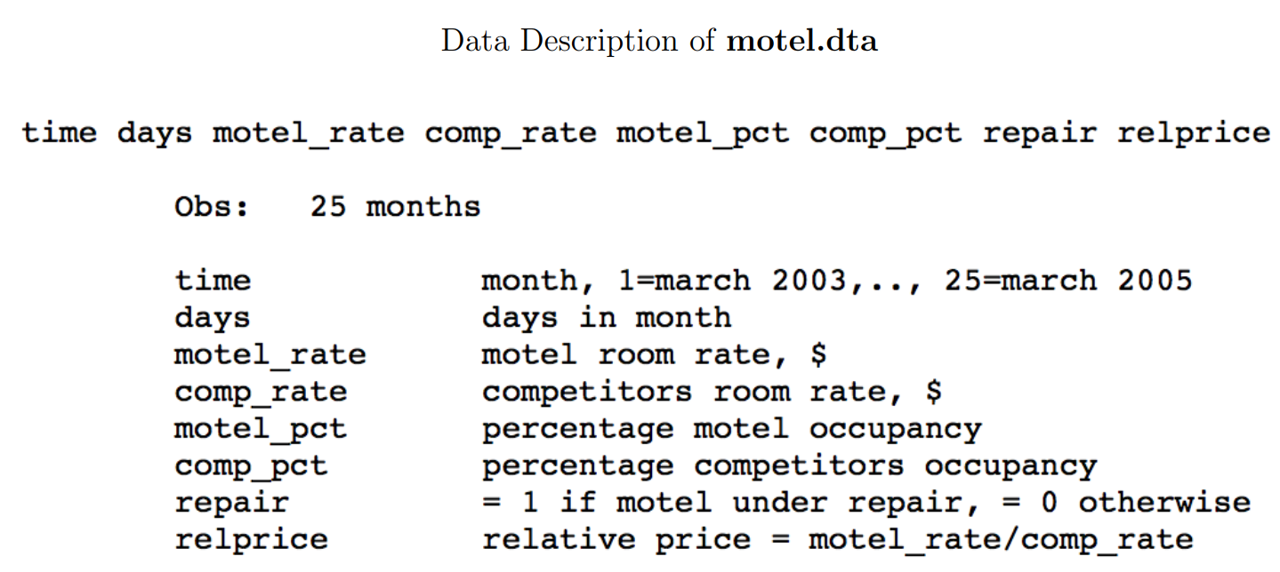
\includegraphics[scale=0.35]{DataDes.png}
    \caption{}
    \label{fig:my_label}
\end{figure}
\end{frame}
%---------------------------------------------------------

%---------------------------------------------------------
\begin{frame}[fragile,t]
\begin{enumerate}[(a)]
    \item Plot $motel\_pct$ and $comp\_pct$ versus $time$ on the same line graph.\\
    What can you say about the occupancy rates over time?\\ 
    Do they tend to move together? 
    %Which had the higher occupancy before the repair period? Which had the higher occupancy during the repair period?
\vspace{4mm}
\end{enumerate}
\pause
\begin{figure}[h]
    \centering
    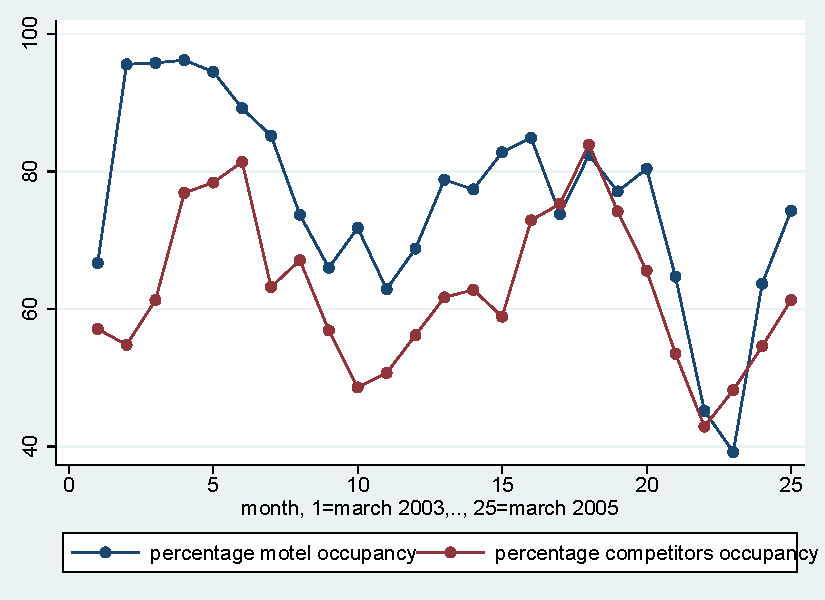
\includegraphics[scale=0.6]{Graph1.pdf}
    \caption{}
    \label{fig:my_label}
\end{figure}
\end{frame}
%---------------------------------------------------------

%---------------------------------------------------------
\begin{frame}[fragile,t]
\begin{enumerate}[(b)]
    \item Plot $motel\_pct$ against $comp\_pct$.\\
    Does there seem to be a relationship between these two variables?\\
    Explain why such a relationship might exist.
\end{enumerate}
\pause
\vspace{4mm}
\begin{figure}[h]
    \centering
    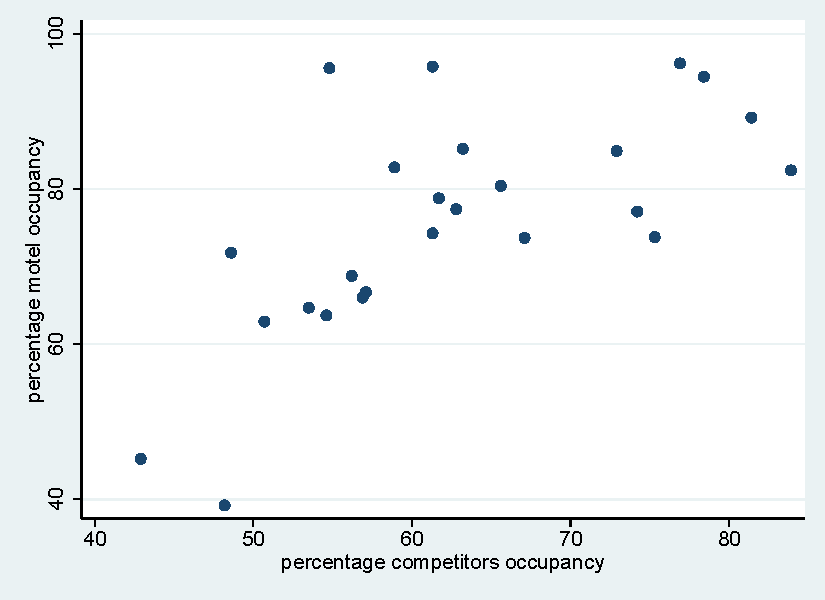
\includegraphics[scale=0.6]{Graph2.pdf}
    \caption{}
    \label{fig:my_label}
\end{figure}
\end{frame}
%---------------------------------------------------------

%---------------------------------------------------------
\begin{frame}[fragile,t]
\begin{enumerate}[(c)]
    \item Estimate the regression model $motel\_pct_t = \beta_0 + \beta_1 comp\_pct_t + u_t$\\
    with (i) homoskedastic-only standard errors\\
    and (ii) heteroskedastic-robust standard errors. \\
    Compare your results.\\
    \pause
    \vspace{10mm}
    \textit{Answer.} The estimated model
    \begin{itemize}
        \item with homoskedastic standard errors is:
        $$\underset{(se)}{\widehat{motel\_pct}} = \underset{(12.9069)}{21.4000} +  \underset{(0.2027)}{0.8646} \cdot comp\_pct \quad R^2=0.4417 \quad SER=11.019$$ 
        %$$\widehat{wage} = -10.4000 + 2.3968 \cdot educ$$ 
        %(Standard errors in parenthesis)	\\
        \item with heteroskedastic-robust standard errors is:
        $$\underset{(se)}{\widehat{motel\_pct}} = \underset{(14.5600)}{21.4000} +  \underset{(0.2160)}{0.8646} \cdot comp\_pct \quad R^2=0.4417 \quad SER=11.019$$ 
    \end{itemize}
\end{enumerate}
\end{frame}
%---------------------------------------------------------

%---------------------------------------------------------
\begin{frame}[fragile,t]
\begin{enumerate}[(d)]
    \item Compute the least squares residuals from the regression in (b).\\
    Plot the residuals against $time$. 
    \\ Does the model over-predict or under-predict the motel’s occupancy rates for the months of repair: $times = 17,18,...,23$?
\end{enumerate}
\pause
\vspace{3mm}
\begin{figure}[h]
    \centering
    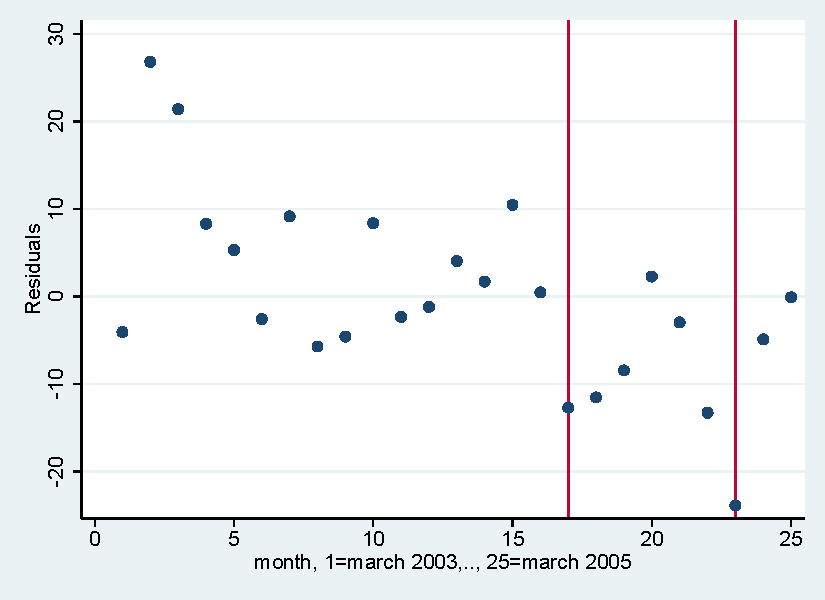
\includegraphics[scale=0.6]{Graph3.pdf}
    \caption{}
    \label{fig:my_label}
\end{figure}
\end{frame}
%---------------------------------------------------------

%---------------------------------------------------------
\begin{frame}[fragile,t]
\begin{enumerate}[(e)]
    \item Create a new variable $relprice100$ which is the ratio of the price per room charged by the motel in question relative to its competitors multiplied by 100.\\  Estimate the regression model $motel\_pct_t = \gamma_0 + \gamma_1 relprice100_t + e_t$. \\
    What is the predicted sign of the slope coefficient $\gamma_1$? \\
    Does the sign of the estimated slope agree with your prediction?\\
    %\item Test the null hypothesis $H_0:\beta_1 = 0$ against the alternative hypothesis $H_1: \beta_1 > 0$ at $\alpha = 0.01$ level of significance. Discuss your conclusion. Clearly define the $t$-statistic used, rejection rule and $p$-value.
    %\item Test the null hypothesis $H_0:\beta_1 = 1$ against the alternative hypothesis $H_1: \beta_1 \neq 1$ at the $\alpha = 0.01$ level of significance. If the null hypothesis were true, what would that imply about the motel’s occupancy rate versus their competitor’s occupancy rate? Discuss your conclusion. Clearly define the $t$-statistic used, rejection rule and $p$-value.
\pause
\vspace{10mm}
\textit{Answer.}
\begin{equation*}
    \underset{(se)}{\widehat{motel\_pct}} = \underset{(42.8497)}{166.6561} -  \underset{(0.5825)}{1.2212} \cdot relprice
\end{equation*}
\begin{equation*}
    R^2=0.160 \quad SER=13.515
\end{equation*}
\end{enumerate}
\end{frame}
%---------------------------------------------------------

%---------------------------------------------------------
\begin{frame}[fragile,t]
\begin{enumerate}[(f)]
    \item Calculate the sample average occupancy rate for the motel\\
    (i) during the time when there were no repairs being made, and \\
    (ii) during the time when there were repairs being made? \\
    How big a difference is there?\\
    %\item Construct a 95\% interval estimate for the parameter $\beta_2$. Have we estimated the association between $motel\_pct$ and $comp\_pct$ relatively precisely, or not? Explain your reasoning.
    %\item  Construct a 90\% interval estimate of the expected occupancy rate of the motel in question, $MOTEL_PCT$, given that $COMP_PCT = 70$.
    \pause
    \vspace{10mm}
    \textit{Answer.}
    The average motel occupancy rate
    \begin{itemize}
        \item during the 18 time periods when no repairs were being made: 79.35\%
        \item during the 7 time periods when repairs were being made: 66.11\%
    \end{itemize}
 $\Rightarrow$ A reduction of 13.24\%
\end{enumerate}
\end{frame}
%---------------------------------------------------------

%---------------------------------------------------------
\begin{frame}[fragile,t]
\begin{enumerate}[(g)]
    \item Consider the linear regression $motel\_pct_t = \delta_0 + \delta_1 repair_t + \epsilon_i$, \\
    where $repair$ is an dummy variable taking the value 1 during the repair period and 0 otherwise. \\
    What are the estimated coefficients?\\ How do these estimated coefficients relate to the calculations in (f)?\\
    %Is this difference statistically significant at $\alpha = 0.10$ level of significance?
    %\item Estimate the regression model $motel\_pct = \beta_0 + \beta_1 comp\_pct + \beta_2 motel\_rate +u$ with heteroskedastic-robust standard errors.  Compare the estimated coefficient for $comp\_pct$ to your answer in part (b).
\pause
\vspace{10mm}
\textit{Answer.}
\begin{equation*}
    \underset{(se)}{\widehat{motel\_pct}} = \underset{(2.7812)}{79.3500}   \underset{(6.9245)}{-13.2357} \cdot repair 
\end{equation*}
\begin{equation*}
    R^2=0.1765 \quad SER=13.38
\end{equation*}
\end{enumerate}

$\hat{u_i} = Y_i - \hat{\beta_0} - \hat{\beta_1}X_i$ = Y_i - \hat{Y_i}$\\
\vspace{3mm}
\textbf{Over-predict}: $\hat{Y_i} > Y_i \Leftrightarrow \hat{u_i} < 0$ (\textbf{Negative} residual)\\
\vspace{3mm}
Under-predict: $\hat{Y_i} < Y_i \Leftrightarrow \hat{u_i} > 0$ (\textbf{Positive} residual)
\end{frame}
%---------------------------------------------------------
%---------------------------------------------------------
\begin{frame}[fragile,t]
\begin{equation*}
motel\_pct_t = \delta_0 + \delta_1 repair_t + \epsilon_i
\end{equation*}
where:
\begin{equation*}
 repair_t= \begin{cases} 0, & \mbox{if the motel is not repaired at t} \\ 1, & \mbox{if the motel is repaired at t}
\end{cases}  
\end{equation*}

\vspace{3mm}

Interpretation of $\delta_0$:  \textcolor{red}{population mean} occupancy rate in the motel when repairs being made.\\ 
\begin{equation*}
   \delta_0 = E(motel\_pct_t|repair_t = 0) 
\end{equation*}

Interpretation of $\delta_1$: The difference in \textcolor{red}{population mean} occupancy rate in the motel between when there were repairs being made and when no repairs were being made. 
\begin{equation*}
   \delta_1 = E(motel\_pct_t|repair_t = 1) - E(motel\_pct_t|repair_t = 0) 
\end{equation*}
\end{frame}
%---------------------------------------------------------

%---------------------------------------------------------
\begin{frame}[fragile,t]
Interpretation of $\hat{\delta_0} = 79.35$: The average motel occupancy rate when no repairs were being made is $79.35\%$

\vspace{3mm}

Interpretation of $\hat{\delta_1} = -13.2357$: The difference in average motel occupancy rate between when there were repairs being made and when no repairs were being made is $-13.2357\%$.

\end{frame}
%---------------------------------------------------------
\end{document}